% -*- coding: utf-8 -*-
\documentclass[UKenglish,12pt]{article}
\usepackage[utf8]{inputenc}
\usepackage[T1]{fontenc,url}
%usepackage newcent for thik text
%\usepackage{babel,csquotes,textcomp}
\usepackage[top=2cm,bottom=2cm,left=2.2cm,right=2.2cm]{geometry}
%\usepackage{float}%Force figur in front of text with H - option
\usepackage{graphicx}
\usepackage{tabulary}
\usepackage{verbatim}
\usepackage{listings}
%\usepackage{bookmark} %also loads package{hyperref}
%removes: Package rerunfile check Warning: File `Essay.out' has changed.
\usepackage{bookmark}
\usepackage{float}

\title{Project 2 - Report - INF4121/3121} % Title
\date{\today} % Date for the report
\author{Sebasting Søberg(INF4121) \& Thomas Oddsund(INF3121)}

% Enumerate in enumerate with numbers instead of letters
\renewcommand{\labelenumii}{\theenumii}
\renewcommand{\theenumii}{\arabic{enumii}.}

%post condition vs expected results: http://www.klaros-testmanagement.com/en/forum/-/message_boards/message/144168


\begin{document}
\maketitle % Insert the title, author and date

\section{Requirement 1}
\subsection{Test cases}
We use state diagram to describe every use-case. When analyzing the use cases we assumed that all the observable results relate to the demo store, and for that reason every time a user gets an email it's under Expected results instead of post-conditions.

\begin{itemize}%all manual test cases
\item[*]
\begin{figure}[!htbp]
\textbf{1.\newline}
\centering
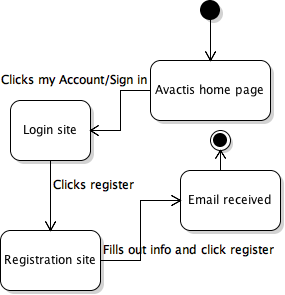
\includegraphics[scale=0.7,keepaspectratio]{Images/CreateAccount.png}
\caption{Create Account}
\end{figure}

\begin{table}[!htbp]
\small
\begin{tabular}{| p{5cm} | p{10cm} | }
	\hline
	\textbf{Type} & \textbf{Description} \\ \hline
	 Title & Create account\\ \hline
	 Objective & To create a valid account that can be used for online shopping on \href{http://demo.avactis.com/4.7.9/}{\textbf{this site}.} \\ \hline
	 Pre-conditions & User has Email\\ \hline
	 Steps & \begin{enumerate} \item User goes to Avactis shopping site \item User clicks \textit{My account or  Sign in} in the top right corner. \item User clicks register \item User fills in necessary information and clicks register after.\end{enumerate} \\ \hline
	 Post-conditions & \begin{enumerate} \item Website says the following in a green field: \textit{Account created successfully. You are now registered.} \item \textit{Sign in} changes to \textit{sign out} \end{enumerate}\\ \hline
	 Expected results & \begin{enumerate} \item User registered in avactis user database. \item User gets a verification email \item User is now logged in \end{enumerate}\\ 
	 \hline
\end{tabular} % & \\ \hline
\end{table}

\item[*]
\begin{figure}[!htbp]
\textbf{2.\newline}
\centering
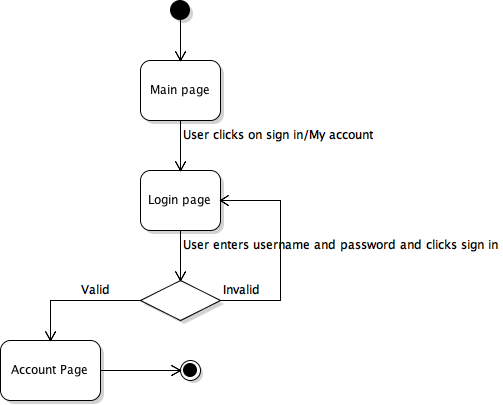
\includegraphics[scale=0.7,keepaspectratio]{Images/Login.png}
\caption{Login}
\end{figure}



\begin{table}[!htbp]
\small
\begin{tabular}{| p{5cm} | p{10cm} | }
	\hline
	\textbf{Type} & \textbf{Description} \\ \hline
	 \textbf{Title} & Logging in\\ \hline
	 \textbf{Objective} & To verify that a user is registered by logging in\\ \hline
	 \textbf{Pre-conditions} & The user has a valid account\\ \hline
	 \textbf{Steps} & \begin{enumerate} \item A user opens a browser and goes to the website \item A user clicks \textit{sign in/my account} in the top right corner. \item The user fills in login details and clicks sign in \end{enumerate} \\ \hline
	 \textbf{Post-conditions} & \begin{enumerate} \item The user has an ongoing session with the shopping website \item The \textit{My Account} page is loaded \item the website changes from the title \textit{sign in} in the top right corner to \textit{sign out} \end{enumerate} \\ \hline
	 \textbf{Expected results} & The user has an active session  \\ 
	 \hline
\end{tabular} % & \\ \hline
\end{table}

\item[*]
\begin{figure}[!htbp]
\textbf{3.\newline}
\centering
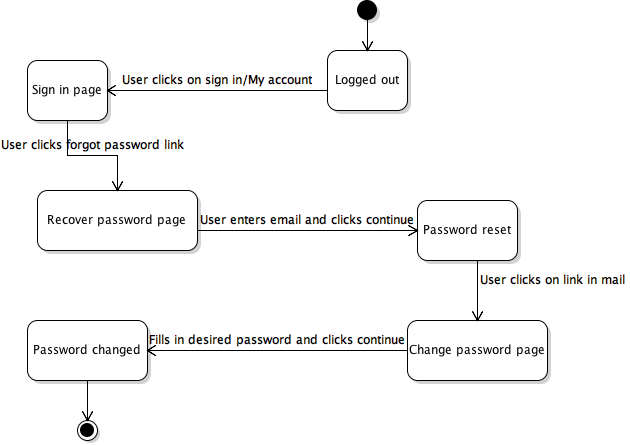
\includegraphics[scale=0.7,keepaspectratio]{Images/ResetPassword.png}
\caption{Reset Password}
\end{figure}

\begin{table}[!htbp]
\small
\begin{tabular}{| p{5cm} | p{10cm} | }
	\hline
	\textbf{Type} & \textbf{Description} \\ \hline
	 \textbf{Title} & Reset Password\\ \hline
	 \textbf{Objective} & To change or alter you password\\ \hline
	 \textbf{Pre-conditions} & A user account on avactis website\\ \hline
	 \textbf{Steps} & \begin{enumerate} \item A user opens a browser and goes to the avactis site \item The user clicks \textit{My account or Sign in} \item The under the login fields the user press the link \textit{Forgot your password?} \item The user then enters their email and click continue \item The user then clicks on the reset link in their email \item Finally the user enter their new passord \end{enumerate} \\ \hline
	 \textbf{Post-conditions} & \begin{enumerate} \item A message pops up in green with: \textit{Your password has been reset. Further instructions have been sent to the e-mail address you provided during registration.} \item After entering a new password \textit{Password saved successfully.} pops up \end{enumerate}\\ \hline
	 \textbf{Expected results} & \begin{enumerate} \item User gets email with link to change password. \item User has a active session after entering new password \end{enumerate} \\ 
	 \hline
\end{tabular} % & \\ \hline
\end{table}

%\begin{enumerate} \end{enumerate}
\item[*]
\begin{figure}[!htbp]
\textbf{4.\newline}
\centering
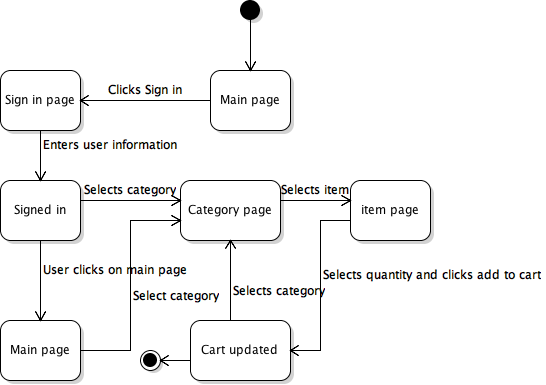
\includegraphics[scale=0.7,keepaspectratio]{Images/SelectProducts.png}
\caption{Select Products}
\end{figure}


\begin{table}[!htbp]
\small
\begin{tabular}{| p{5cm} | p{10cm} | }
	\hline
	\textbf{Type} & \textbf{Description} \\ \hline
	 \textbf{Title} & Select Products \\ \hline
	 \textbf{Objective} & Put different products in the cart and manage the quantity of each item \\ \hline
	 \textbf{Pre-conditions} & User has avactis account \\ \hline
	 \textbf{Steps} & \begin{enumerate} \item Go to main page and click \textit{Sign in/My Account} \item Fill in username and password and click sign in \item Select categories to shop from \item Select one or more products and their quantity.
	 \end{enumerate} \\ \hline
	 \textbf{Post-conditions} & \begin{enumerate} \item Item and price counter changes \item Cart contains products \end{enumerate}  \\ \hline
	 \textbf{Expected results} & Cart contains products \\ 
	 \hline
\end{tabular} % & \\ \hline
\end{table}


\item[*] % basically this test case and diagram shall cover 3-5
\begin{figure}[!htbp]
\textbf{5.\newline}
\centering
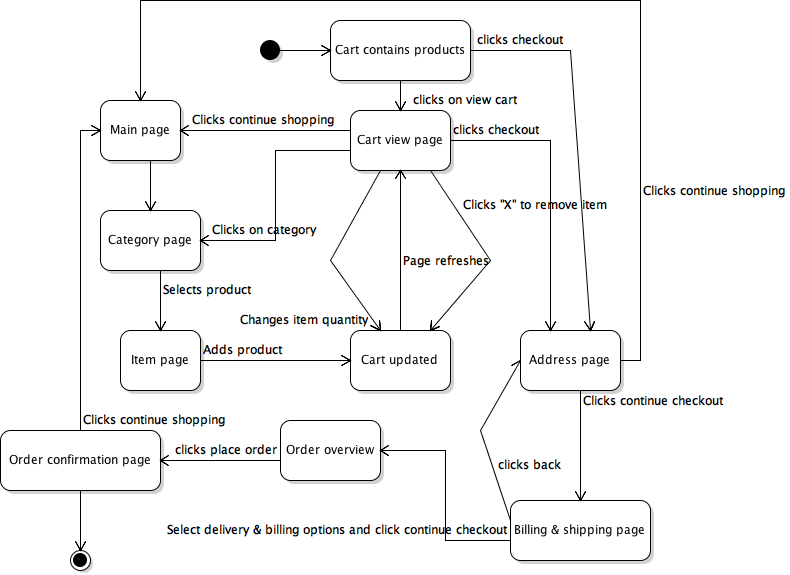
\includegraphics[scale=0.60,keepaspectratio]{Images/BuyProductsandChangeCart.png}
\caption{Manage shopping cart, change quantity and place order}
\end{figure}

\begin{table}[!htbp]
\small
\begin{tabular}{| p{5cm} | p{10cm} | }
	\hline
	\textbf{Type} & \textbf{Description} \\ \hline
	 \textbf{Title} & Shopping cart management, Checkout, products quantity, add/remove items and purchasing \\ \hline
	 \textbf{Objective} & Test that the cart indeed contains the chosen products after shopping session \\ \hline
	 \textbf{Pre-conditions} & Avactis user account and a cart of products \\ \hline
	 \textbf{Steps} & \begin{enumerate} \item Click View cart \item Change items quantity \item Add/remove product(s) \item a Click checkout \item Fill in Billing \& shipping address and click continue checkout \item Select Billing and delivery options \item Click place order
	 \end{enumerate} \\ \hline
	\textbf{Post-conditions} & \begin{enumerate}\item Item and price counter changes \item Website states goes to order confirmation page \item Webpage with following message: \textit{Your order is placed. Order ID: \#00001 Order details have been sent to your e-mail address.}  \end{enumerate} \\ \hline
	 \textbf{Expected results} & \begin{enumerate}\item Users gets order confirmation mail \item Cart is empty \item Item and money counter is zero initialized \end{enumerate}\\ 
	 \hline
\end{tabular} % & \\ \hline
\end{table}
%TODO: Include x button right from shopping draw menu in cart "menu"

\item[*]
\begin{figure}[!htbp]
\textbf{6.\newline}
\centering
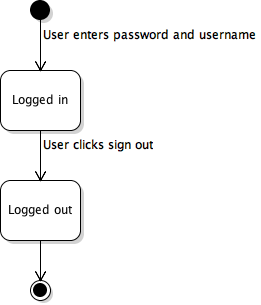
\includegraphics[scale=0.6,keepaspectratio]{Images/Logout.png}
\caption{Logout}
\end{figure}


\begin{table}[!htbp]
\small
\begin{tabular}{| p{5cm} | p{10cm} | }
	\hline
	\textbf{Type} & \textbf{Description} \\ \hline
	 \textbf{Title} & Logout \\ \hline
	 \textbf{Objective} & To log out of Avactis webstore \\ \hline
	 \textbf{Pre-conditions} & A user account \\ \hline
	 \textbf{Steps} & \begin{enumerate} \item Go to Avactis homepage and click sign in \item Enter password and username \item click logout  \end{enumerate}\\ \hline
	 \textbf{Post-conditions} & \begin{enumerate}\item\textit{Sign in} changes to \textit{sign out} \item The active session is ended on the website \end{enumerate}  \\ \hline
	 \textbf{Expected results} & The user is logged out\\ 
	 \hline
\end{tabular} % & \\ \hline
\end{table}


\end{itemize}

\newpage
\subsection{Error Report}
CSS module fails to load. We used \href{http://www.uio.no/studier/emner/matnat/ifi/INF3121/v16/resources/1-lectures/l05.pdf}{this} report and left out those field which didn't apply for us.

%Also this: http://demo.avactis.com/4.7.9/avactis-themes/metro/css/bootstrap.css.map fails to load on every single page
%Unused fields: change history, References and incident resolution
%Bug: if user clicks "forgotten password", the account is deactivated untill link in the mail has been clicked. This means that users who accidently delete the mail are locked out


\begin{center}
\begin{table}[!htbp]
\small
\begin{tabular}{| p{3.8cm} | p{5cm} | p{3.4cm} | p{4cm} |}
	\hline
	 \textbf{Date:} & \date{\today} & \textbf{Project:} & \textit{INF3121 Project2}\\ \hline
	 \textbf{Programmer:} & \textit{Sebastian Søberg} & \textbf{Tester:} & \textit{Sebastian Søberg} \\ \hline
	 \textbf{Program/Module:} & \textit{\href{http://demo.avactis.com/4.7.9/index.php}{Avactis Demo webstore}} & \textbf{Build/Release:} & \textit{4.7.9} \\ \hline
	 \multicolumn{1}{| p{5cm} |}{\textbf{Software enviroment:}} & \multicolumn{3}{| p{10cm} |}{\textit{\textbf{OS:} Mac OS X El Captian. \textbf{Browser:} Safari v9.1}}  \\ \hline
	 \multicolumn{1}{| p{5cm} |}{\textbf{Hardware enviroment:}} & \multicolumn{3}{| p{10cm} |}{\textit{Model: Macbook air mid 2012, RAM: 4gb, CPU: 1,8 GHz Intel Core i5, Graphics: Intel HD Graphics 4000 1536 MB}}  \\ \hline
	 \textbf{Status of incident:} & \textit{Not fixed} & \textbf{Number of occurences} & \textit{Every page load} \\ \hline
	 \textbf{Severity:} & \textit{Medium} & \textbf{Impact:} & \textit{CSS module not loaded} \\ \hline
	 \textbf{Priority} & \textit{Medium} & \textbf{Expected result:} & \textit{Every page generated by avactis web store would load without an error.} \\ \hline
	 \multicolumn{1}{| p{5cm} |}{\textbf{Detailed Description:}} & \multicolumn{3}{| p{10cm} |}{\textit{On every page-load in the webstore it has an error when trying to load http://demo.avactis.com/4.7.9/avactis-themes/metro/css/bootstrap.css.map. This results in 102 CSS warnings at the home page only}}  \\ \hline
	 \textbf{Assigned to:} & \multicolumn{3}{| p{10cm} |}{\textit{Raluca Florea - University Of Oslo}} \\
	 \hline
\end{tabular} 
\end{table}
\end{center}
%\textbf{} & \textit{} & \textbf{} & \textit{} \\ \hline
\pagebreak
\section{Requirement 2}
\subsection{About the ordering of the tests}
The order of the test is described in this dependancy graph:

\begin{figure}[!htbp]
	\centering
	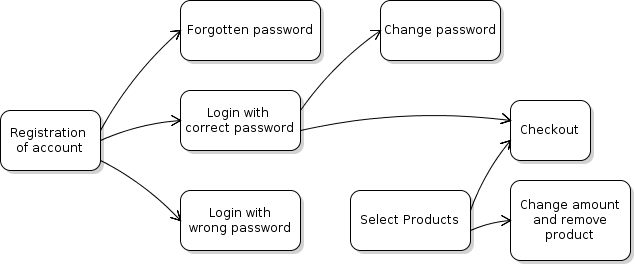
\includegraphics[scale=0.6,keepaspectratio]{Images/dependancygraph.png}
	\caption{Dependancy graph}
\end{figure}

This shows that the way we have set up the tests, some ordering is absolute. I.e. to ensure that we are logging into an account with a wrong password, there need to exist an account where we know the correct password. The same goes for forgotten password. When it comes to checkout, this can be done without logging in, but we have designed the tests with a logged in user in mind, so that the customer info is fetched automatically. The result is the dependancy graph shown above, where arrow in means that it's dependant on the test the arrow originates from, while arrow out signals another test is dependant on it.

\vspace{0.5cm}
\href{https://github.com/sebasso/INF4121-Project2}{\textbf{\Large{Github Link}}}

\begin{figure}[H]
	\centering
	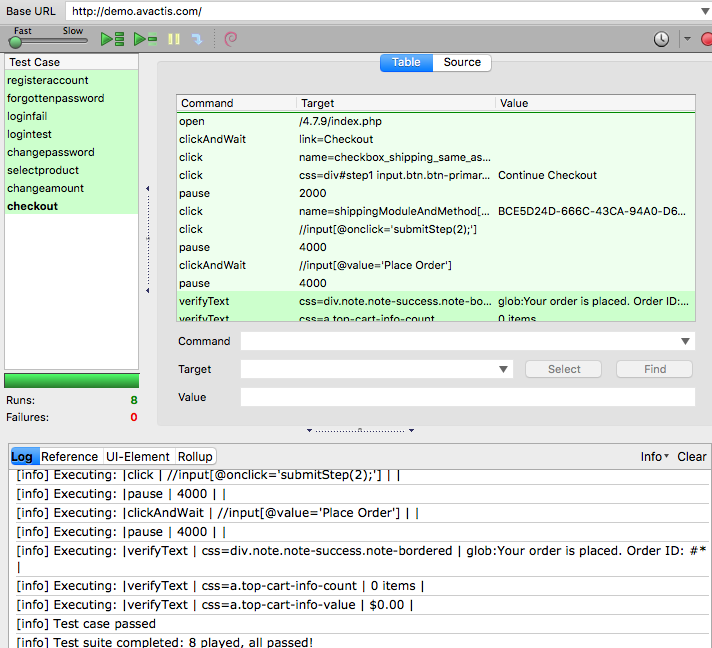
\includegraphics[scale=0.7,keepaspectratio]{Images/Selenium-screenshot.png}
	\caption{Selenium Execution Results\newline NB: \textit{As seen in the picture this taken when every test is passed and marked in green. Ergo it works correctly}}
\end{figure}


\section{Requirement 3}
We had Total coverage of every manual test in our automated testing suite. However we couldn't do this with only bare-bone recording. We needed to manually configure the following tests:



\end{document}